\chapter[THIẾT KẾ HỆ THỐNG]{THIẾT KẾ VÀ PHƯƠNG PHÁP LUẬN TRIỂN KHAI HỆ THỐNG PHÁT HIỆN TÉ NGÃ}
\label{chap:methodology} % Chapter label for cross-referencing (consistent English style)

\section*{} % Chapter introduction (un-numbered section)
% This section serves as the transition from the theoretical background (Chapter 2) to the system implementation.
Chương trước đã thiết lập nền tảng lý thuyết toàn diện về các công nghệ cốt lõi. Chương này sẽ tập trung vào việc kiến trúc hóa và chi tiết hóa hệ thống phát hiện té ngã tích hợp. Nội dung chương sẽ mô tả chi tiết \textbf{kiến trúc tổng thể} của hệ thống đa phương thức, các lựa chọn phần cứng và phần mềm nhúng, cách thức thiết kế thuật toán nhận diện té ngã (Detection Logic), và quy trình triển khai hệ thống cảnh báo thời gian thực. Chương 3 đóng vai trò là cầu nối từ nghiên cứu cơ sở đến ứng dụng thực tiễn của \TENLUANVAN.

% --- START OF CHAPTER SECTIONS (Input files) ---
\section{1 System Architecture}
 % 3.1 System block diagram and overall design


\section{Thực hiện phần cứng}
\label{sec:hardware_implementation}

Hệ thống Phát hiện té ngã và Cảnh báo (FDAS) được triển khai theo kiến trúc mô-đun với hai module chính hoạt động độc lập, đảm bảo linh hoạt, khả năng giám sát rộng và duy trì hoạt động khi một module gặp sự cố. Module I tập trung vào thu thập dữ liệu chuyển động và định vị, trong khi Module II xử lý hình ảnh để xác nhận sự kiện té ngã.

\subsection{Module I: Thiết bị đeo / Cảm biến}
\label{ssec:module_one}

Module I là thiết bị phát hiện ban đầu, thiết kế nhỏ gọn để người dùng mang theo. Các thành phần chính bao gồm:

\begin{figure}[H]
    \centering
    \includegraphics[width=0.7\textwidth]{figures/module1_block_diagram-crop.pdf}
    \caption{Sơ đồ khối Module I: Thiết bị đeo / Cảm biến}
    \label{fig:module1_block_diagram}
\end{figure}

\begin{itemize}
    \item \textbf{ESP32-DevKitC-1}: Bộ vi điều khiển trung tâm, tích hợp Wi-Fi và Bluetooth, chi phí thấp, hiệu suất ổn định.
    \item \textbf{MPU6050}: Cảm biến IMU 6 trục, đo gia tốc và tốc độ góc, tích hợp bộ xử lý chuyển động DMP.
    \item \textbf{Module GPS/4G (EC800K)}: Thu thập tọa độ GPS và gửi dữ liệu cảnh báo qua mạng 4G.
    \item \textbf{Các thành phần hỗ trợ}: Buzzer và LED onboard để phản hồi tức thì khi phát hiện sự kiện.
\end{itemize}

\begin{figure}[H]
    \centering
    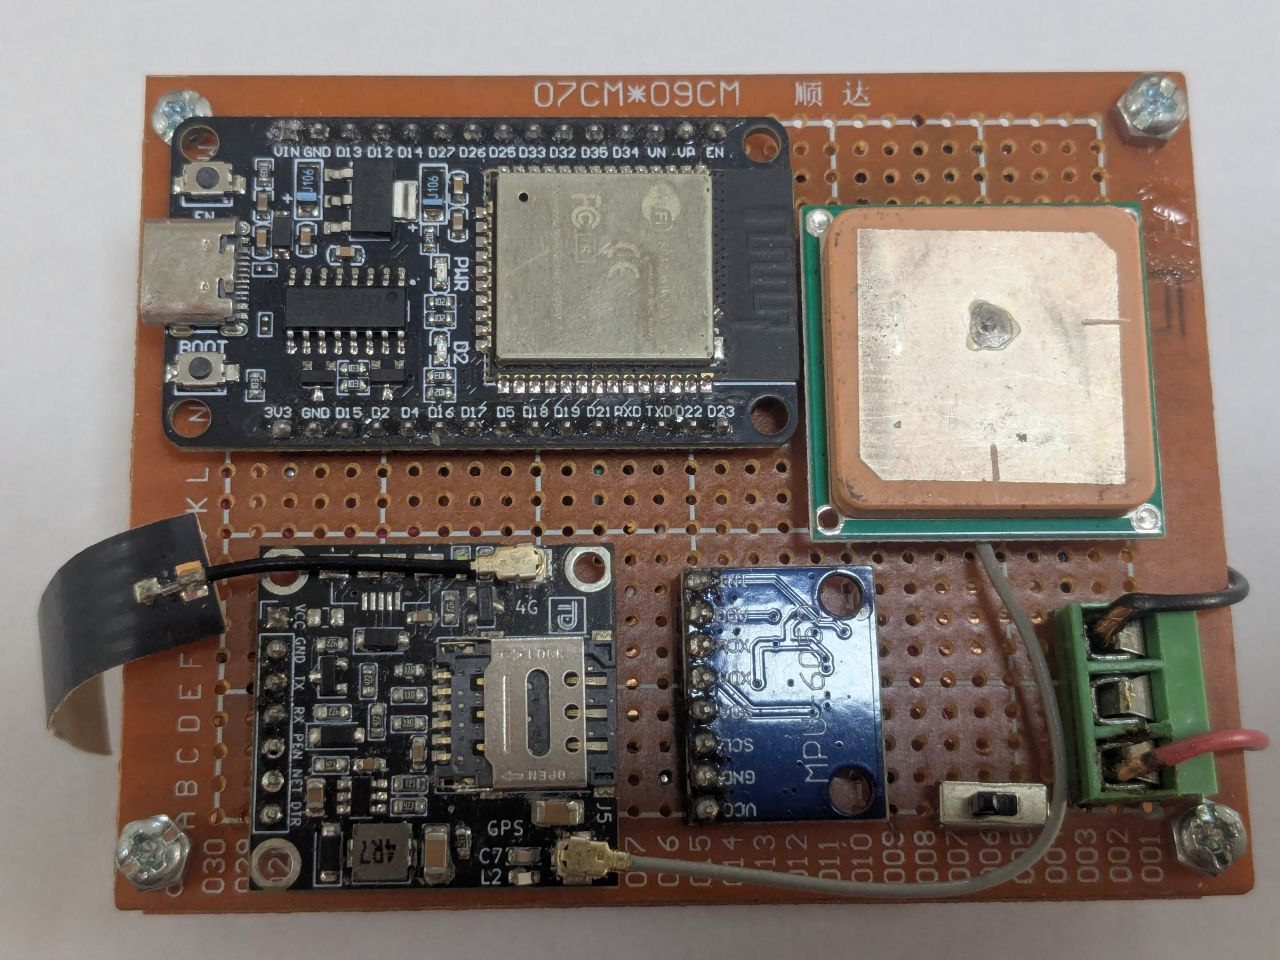
\includegraphics[width=0.8\textwidth]{figures/real_board1.jpg}
    \caption{Hình ảnh thực tế Module I đã hoàn thiện}
    \label{fig:module1_photo}
\end{figure}

Sơ đồ nguyên lý chi tiết (schematic) được vẽ bằng KiCad, đính kèm trong \textbf{Phụ lục B}.

\subsection{Module II: Camera giám sát}
\label{ssec:module_two}

Module II xác nhận sự kiện té ngã bằng hình ảnh, đặt ở khu vực giám sát trọng yếu. Các thành phần chính:

\begin{itemize}
    \item \textbf{ESP32-S3-N16R8}: Vi điều khiển mạnh mẽ, tích hợp Wi-Fi/Bluetooth, hỗ trợ PSRAM và giao diện camera chuyên dụng, tối ưu xử lý luồng dữ liệu hình ảnh.
    \item \textbf{Camera OV5640}: Cảm biến 5MP, hỗ trợ nhiều kích thước khung hình (QQVGA đến UXGA), giao tiếp dữ liệu song song 8-bit với SCCB, xung nhịp 20 MHz.
\end{itemize}

\paragraph{Sơ đồ kết nối phần cứng}
Bảng \ref{tab:pin_mapping} tóm tắt sơ đồ chân giữa ESP32-S3 và OV5640.

\begin{table}[H]
    \centering
    \caption{Sơ đồ kết nối chân giữa ESP32-S3 và OV5640}
    \label{tab:pin_mapping}
    \begin{tabular}{|l|c|l|}
    \hline
    \textbf{Chức năng} & \textbf{Chân ESP32-S3} & \textbf{Mô tả} \\
    \hline
    XCLK & 15 & Tín hiệu xung nhịp cho camera \\
    SIOD (SDA) & 4 & Dòng dữ liệu I2C \\
    SIOC (SCL) & 5 & Xung nhịp I2C \\
    D0-D7 & 11,9,8,10,12,18,17,16 & Bus dữ liệu 8-bit \\
    VSYNC & 6 & Đồng bộ khung hình dọc \\
    HREF & 7 & Tham chiếu hàng ngang \\
    PCLK & 13 & Xung nhịp điểm ảnh \\
    \hline
    \end{tabular}
\end{table}

\begin{figure}[H]
    \centering
    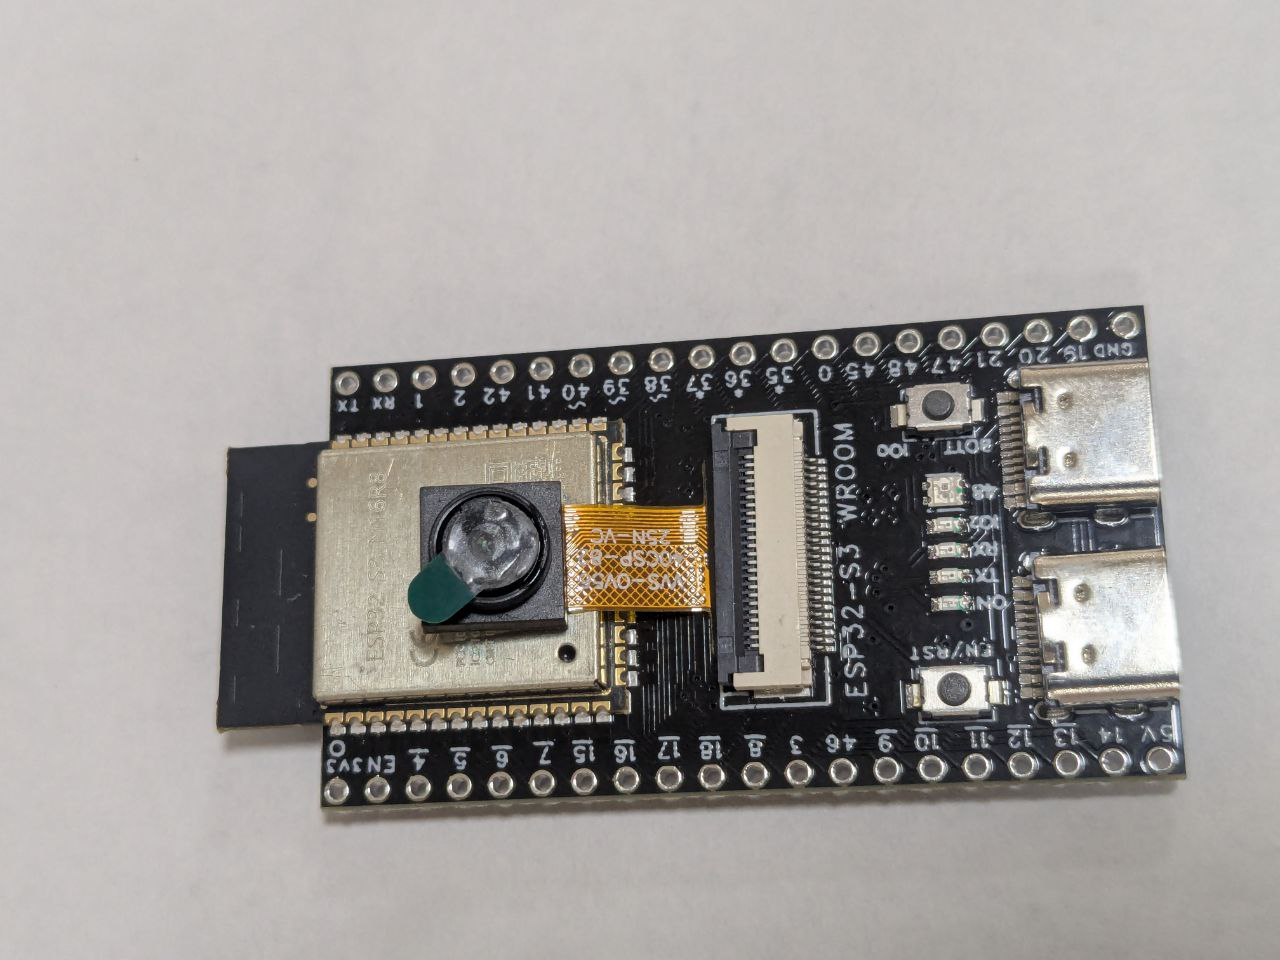
\includegraphics[width=0.8\textwidth]{figures/real_board2.jpg}
    \caption{Hình ảnh thực tế Module II}
    \label{fig:module2_photo}
\end{figure}

\subsection{Bảng tổng hợp các thành phần phần cứng}
\label{ssec:component_summary}

Bảng \ref{tab:hardware_components} tóm tắt các thành phần chính của hai module cùng vai trò và giá thành ước tính.

\begin{table}[H]
    \centering
    \caption{Tổng hợp các thành phần phần cứng}
    \label{tab:hardware_components}
    \begin{tabular}{|l|p{5cm}|p{2cm}|l|}
    \hline
    \textbf{Thành phần} & \textbf{Chức năng} & \textbf{Hình ảnh} & \textbf{Giá thành ước tính (VNĐ)} \\
    \hline
    ESP32-DevKitC-1 & Vi điều khiển chính & 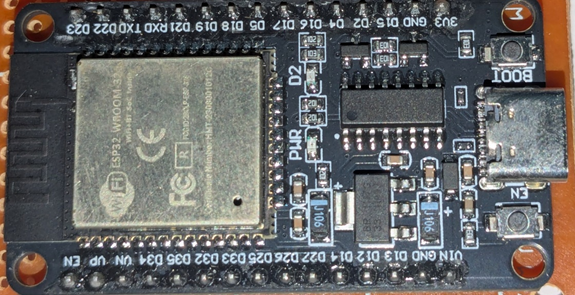
\includegraphics[width=2cm]{figures/real_esp32_c1.png} & 110.000 - 125.000 \\
    MPU6050 & Cảm biến IMU 6 trục & 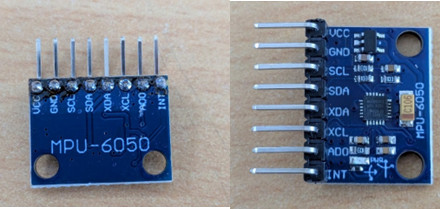
\includegraphics[width=2cm]{figures/real_mpu6050.png} & 45.000 - 55.000 \\
    GPS-antenna & Anten nhận GPS & 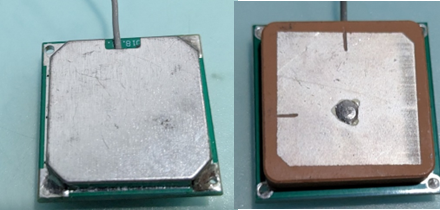
\includegraphics[width=2cm]{figures/real_gps_antenna.png} & 35.000 - 60.000 \\
    Module GPS/4G (EC800K) & Định vị và gửi cảnh báo & 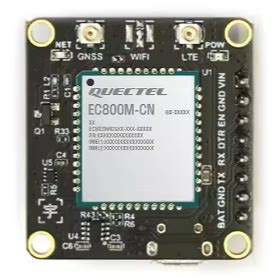
\includegraphics[width=2cm]{figures/real_ec800k.jpg} & ~240.000 \\
    Buzzer & Cảnh báo âm thanh & 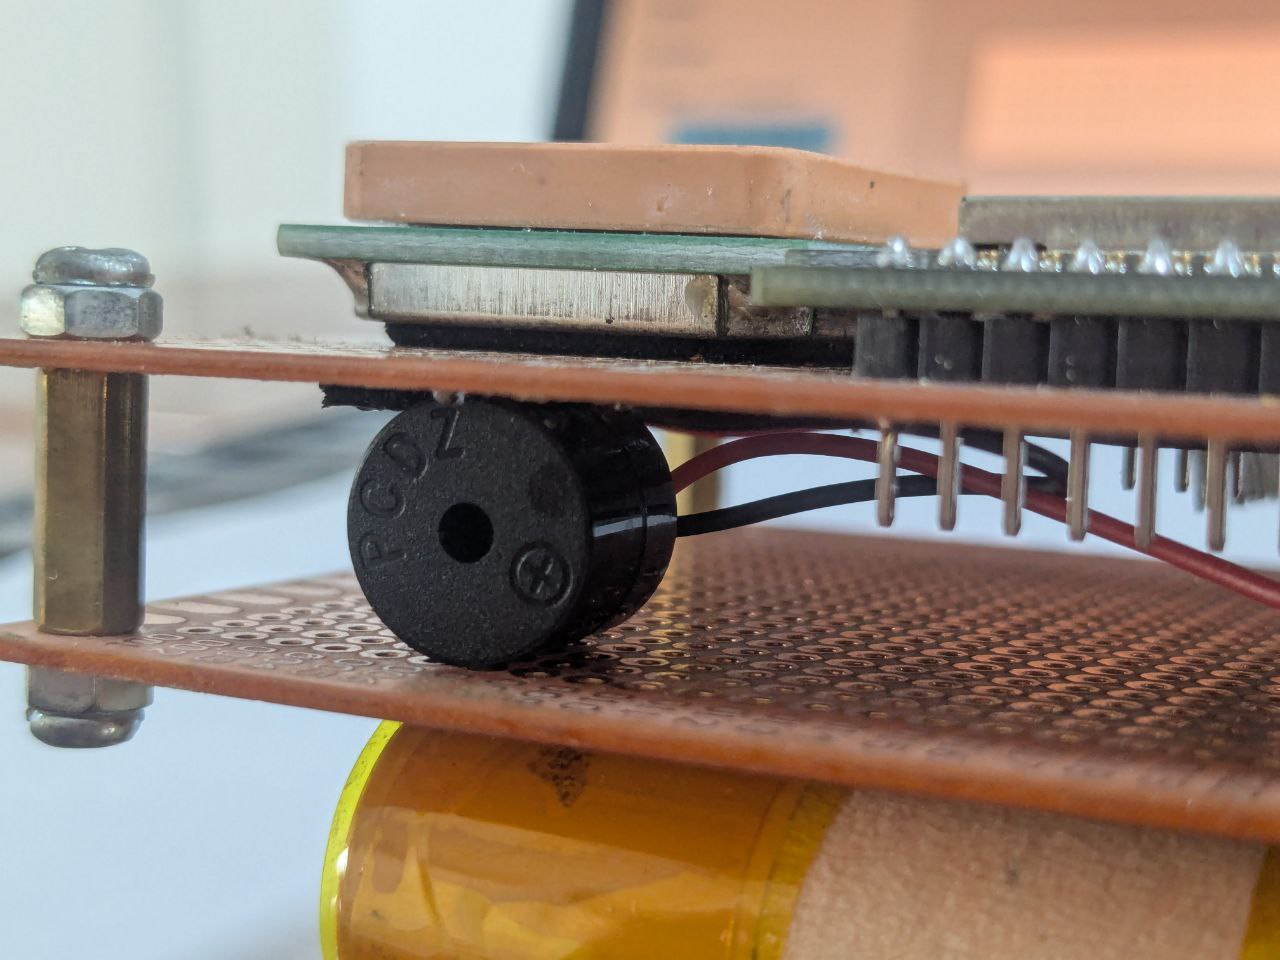
\includegraphics[width=2cm]{figures/real_buzzer.jpg} & 5.000 - 10.000 \\
    ESP32-S3-N16R8 & Vi điều khiển xử lý hình ảnh & 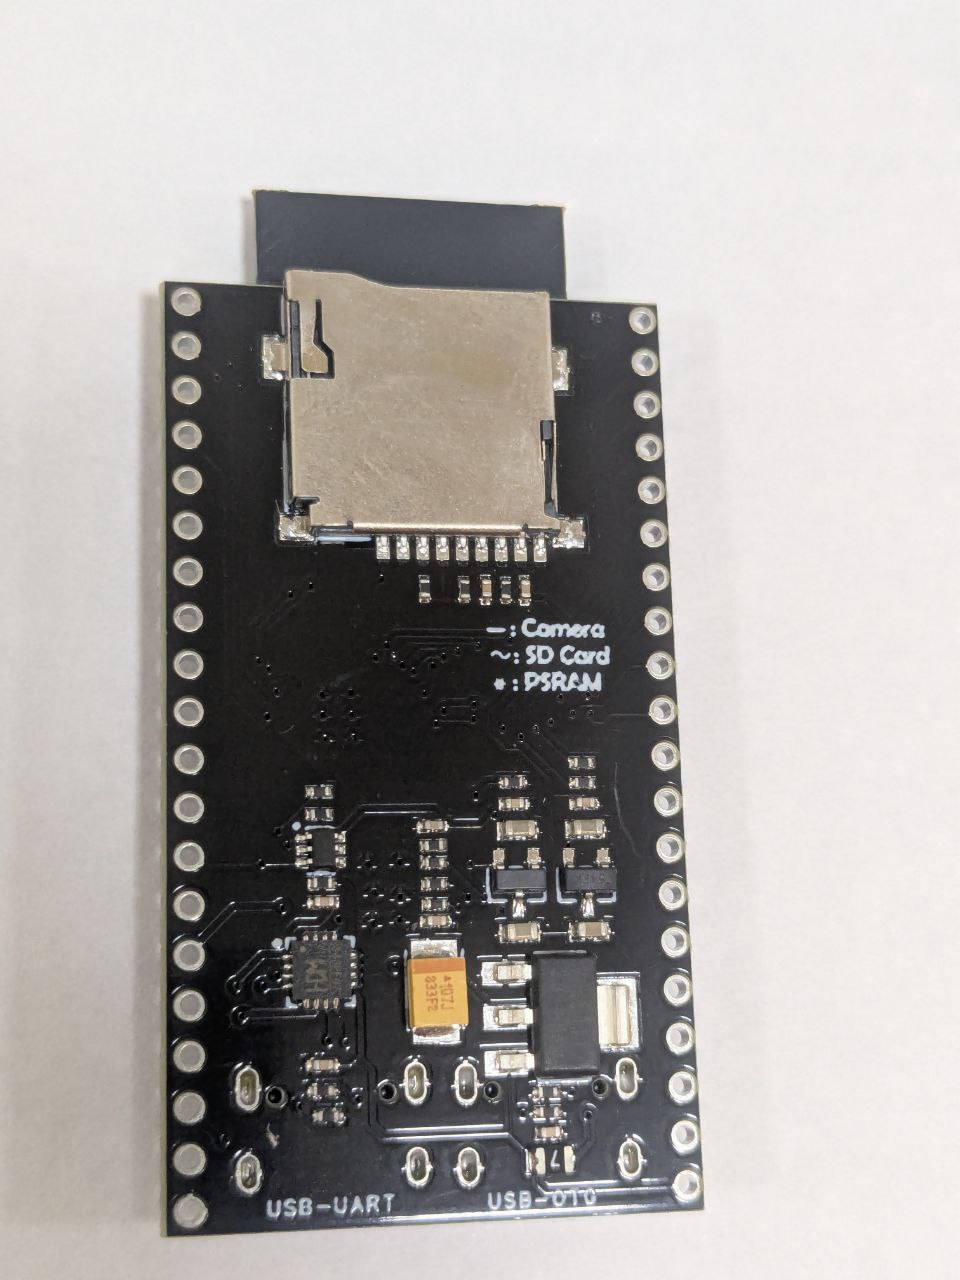
\includegraphics[width=2cm]{figures/real_esp32_s3_2.jpg} & 275.000 - 300.000 \\
    Camera OV5640 & Cảm biến hình ảnh 5MP & 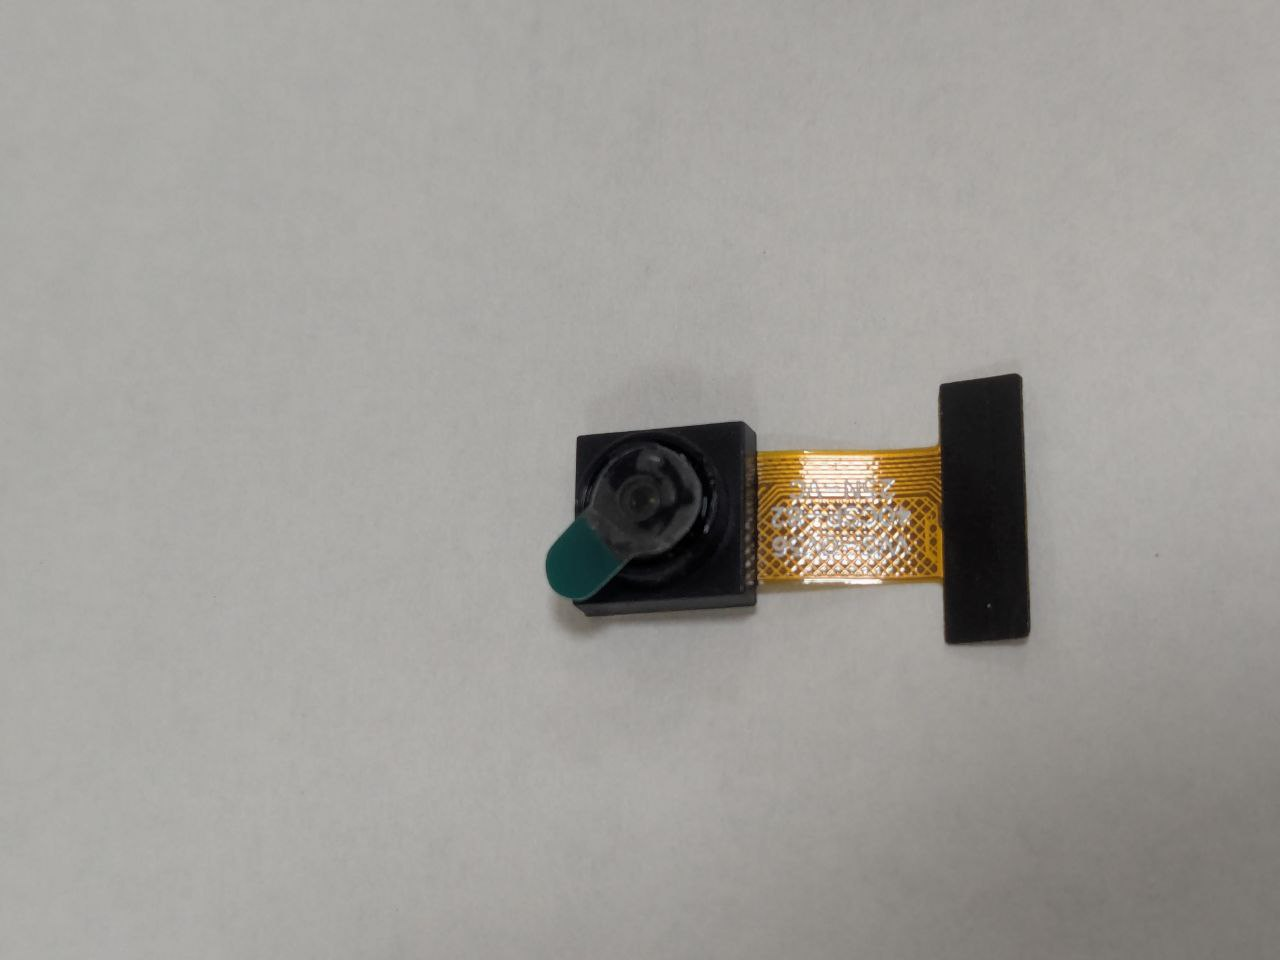
\includegraphics[width=2cm]{figures/real_ov5640.jpg} & 150.000 - 200.000 \\
    \hline
    \end{tabular}
\end{table}
 % 3.2 Details on physical components (ESP32, Camera, IMU)

\section{Triển khai Phần mềm (Software Implementation)}
\label{sec:software_implementation}

Việc triển khai phần mềm được thực hiện theo kiến trúc mô-đun, đảm bảo tính linh hoạt và dễ dàng bảo trì. Các thành phần phần mềm chính bao gồm: mã nhúng cho thiết bị cảm biến và camera, phần mềm xử lý trung tâm trên máy chủ và hệ thống cảnh báo tự động. Mỗi thành phần được phát triển để thực hiện một chức năng cụ thể và giao tiếp với nhau để tạo thành một hệ thống phát hiện té ngã hoàn chỉnh.


\subsection{Mô-đun nhúng phát hiện té ngã (ESP32)}
\label{sec:module_i}

Mô-đun nhúng phát hiện té ngã được triển khai trên nền tảng vi điều khiển ESP32, đóng vai trò là nút cảm biến và trung tâm cảnh báo trong hệ thống. Chức năng chính của mô-đun là thu thập dữ liệu chuyển động từ cảm biến, phân tích thuật toán phát hiện té ngã và kích hoạt cơ chế cảnh báo theo thời gian thực, cả cục bộ (buzzer, LED) và từ xa (Wi-Fi/4G, MQTT, SMS).

\paragraph{Môi trường phát triển}  
Phần mềm được xây dựng trên \textbf{ESP-IDF} (Espressif IoT Development Framework), cung cấp hệ thống build dựa trên \textbf{CMake}, quản lý mô-đun thông qua \texttt{idf\_component.yml}, cũng như các API điều khiển ngoại vi (UART, I2C, SPI, PWM, GPIO) và dịch vụ mạng (Wi-Fi, MQTT, HTTP). Cấu hình dự án sử dụng \textbf{Kconfig}, lưu trữ trong \texttt{sdkconfig}, cho phép tinh chỉnh tham số mà không cần thay đổi mã nguồn. Môi trường này đảm bảo tính ổn định, khả năng mở rộng và tương thích với các driver hiện có.

\paragraph{Luồng làm việc}  
Phần mềm được tổ chức theo một luồng làm việc logic, điều phối từ việc thu thập dữ liệu cảm biến đến xử lý sự kiện và kích hoạt cảnh báo. Sơ đồ minh họa luồng làm việc chính của mô-đun được thể hiện trong Hình~\ref{fig:module1_flow}.

\begin{figure}[h!]
    \centering
    \includegraphics[width=0.8\textwidth, height=0.7\textheight, keepaspectratio]{figures/module1_time_flow.pdf}
    \caption{Lưu đồ luồng làm việc của mô-đun phát hiện té ngã trên ESP32.}
    \label{fig:module1_flow}
\end{figure}

\paragraph{Cấu trúc phần mềm}  
Phần mềm được thiết kế theo kiến trúc \textbf{mô-đun} và \textbf{phân lớp}, đảm bảo tính linh hoạt, mở rộng và dễ bảo trì. Mỗi chức năng được đóng gói thành các thành phần độc lập, từ thu thập dữ liệu, phân tích thuật toán, đến quản lý giao tiếp mạng. Cấu trúc tổng thể dự án:

\begin{minted}[fontsize=\footnotesize, breaklines, frame=single, linenos]{text}
mainproject/
├── main/
│   ├── main.c
│   ├── app_main.c
│   └── app_main.h
├── components/
│   ├── buzzer/
│   ├── comm/
│   ├── data_manager/
│   ├── event_handler/
│   ├── fall_logic/
│   ├── json_wrapper/
│   ├── led_indicator/
│   ├── mpu6050/
│   ├── sim4g_gps/
│   ├── user_mqtt/
│   └── wifi_connect/
\end{minted}

\paragraph{Mô tả các thành phần}
\begin{itemize}
    \item \textbf{main.c}: Điểm khởi đầu, gọi \texttt{app\_main()}.  
    \item \textbf{app\_main.c/h}: Bộ điều phối chính, khởi tạo và liên kết các mô-đun.  
    \item \textbf{fall\_logic}: Thuật toán phát hiện té ngã dựa trên dữ liệu MPU6050.  
    \item \textbf{event\_handler}: Điều phối phản ứng (buzzer, LED, MQTT, SMS).  
    \item \textbf{mpu6050}: Driver cảm biến chuyển động.  
    \item \textbf{buzzer, led\_indicator}: Cảnh báo cục bộ.  
    \item \textbf{sim4g\_gps, wifi\_connect}: Kết nối từ xa, gửi dữ liệu và SMS.  
    \item \textbf{user\_mqtt}: Giao tiếp với máy chủ qua MQTT.  
    \item \textbf{comm, data\_manager}: Quản lý giao tiếp phần cứng và dữ liệu.  
    \item \textbf{json\_wrapper}: Chuẩn hóa dữ liệu trao đổi với hệ thống bên ngoài.
\end{itemize}

\begin{figure}[H]
    \centering
    \includegraphics[width=0.9\textwidth]{figures/module1_software_block-crop.pdf}
    \caption{Sơ đồ khối phần mềm của mô-đun nhúng ESP32.}
    \label{fig:module1_software_block}
\end{figure}

\paragraph{Thuật toán phát hiện té ngã}  
Thuật toán trong \texttt{fall\_logic} sử dụng \textbf{gia tốc tổng hợp}:

\[
a_{total} = \sqrt{a_x^2 + a_y^2 + a_z^2}
\]

Khi $a_{total}$ giảm dưới ngưỡng (\texttt{FALL\_THRESHOLD}), hệ thống đánh dấu sự kiện nghi ngờ té ngã. Ngưỡng có thể hiệu chỉnh qua \texttt{CONFIG\_FALL\_LOGIC\_THRESHOLD\_G}. Thuật toán chạy trong \textbf{tác vụ FreeRTOS riêng biệt} theo chu kỳ \texttt{CHECK\_INTERVAL\_MS}. Trong mỗi chu kỳ:

\begin{enumerate}
    \item Đọc dữ liệu từ \texttt{mpu6050}.  
    \item Tính toán gia tốc tổng hợp và so sánh với ngưỡng.  
    \item Nếu vượt ngưỡng, gửi \texttt{EVENT\_FALL\_DETECTED} tới \texttt{event\_handler}.  
    \item Đặt cờ trạng thái (\texttt{s\_fall\_detected}) để tránh cảnh báo trùng lặp, reset qua \texttt{fall\_logic\_reset\_fall\_status()}.
\end{enumerate}

\begin{figure}[h!]
    \centering
    \includegraphics[width=0.7\textwidth]{figures/module1_fall_logic_diagram.pdf}
    \caption{Lưu đồ thuật toán phát hiện té ngã trong mô-đun \texttt{fall\_logic}.}
    \label{fig:fall_logic_flow}
\end{figure}

\paragraph{Cơ chế biên dịch và cấu hình}  
Mỗi mô-đun trong \texttt{components/} định nghĩa bằng \texttt{CMakeLists.txt} và đăng ký qua \texttt{idf\_component\_register}, quản lý phụ thuộc rõ ràng và chỉ biên dịch mô-đun cần thiết. Tham số hệ thống (UART, mạng, ngưỡng té ngã) được tập trung trong \texttt{Kconfig} và \texttt{sdkconfig}, giúp linh hoạt và hạn chế lỗi khi thay đổi cấu hình.

\paragraph{Tóm tắt}  
Kiến trúc mô-đun cho phép mỗi thành phần đảm nhận chức năng riêng biệt, tăng tính linh hoạt, khả năng mở rộng và dễ bảo trì. Mô-đun nhúng ESP32 thực hiện phát hiện té ngã và cảnh báo theo thời gian thực, đồng thời hỗ trợ cảnh báo cục bộ và truyền dữ liệu tới hệ thống giám sát tổng thể. Đây là nền tảng cho các giai đoạn phát triển tiếp theo, ví dụ thêm cảm biến hoặc mở rộng kênh truyền thông.

\subsection{Module II: Hệ thống Truyền tải Video Thời gian thực (Software Implementation)}
\label{sec:module_ii_software}

\subsubsection{Tổng quan phần mềm}
Phần mềm của Module II được triển khai trên vi điều khiển \textbf{ESP32-S3} để thu thập và truyền tải video từ camera OV5640 theo thời gian thực. Hệ thống hoạt động như một thiết bị đầu cuối thông minh, cung cấp luồng video MJPEG qua HTTP làm nguồn dữ liệu cho các module xử lý thị giác máy tính ở tầng cao hơn.  

Mô hình phần mềm dựa trên kiến trúc **hướng sự kiện (event-driven)** của ESP-IDF, cho phép quản lý đồng thời các tác vụ mạng, camera, và xử lý bộ đệm mà không làm nghẽn luồng.

\subsubsection{Luồng hoạt động chính}
Sơ đồ Hình \ref{fig:sw_architecture_flow} minh họa luồng phần mềm:

\begin{figure}[H]
    \centering
    \includegraphics[width=0.7\textwidth]{module2_flow_2.pdf}
    \caption{Luồng hoạt động chính của phần mềm Module II}
    \label{fig:sw_architecture_flow}
\end{figure}

Các bước chính gồm:

\begin{enumerate}
    \item \textbf{Khởi tạo hệ thống}: cấu hình Wi-Fi, camera, và máy chủ HTTP.
    \item \textbf{Chờ yêu cầu client}: hệ thống liên tục lắng nghe yêu cầu xem video.
    \item \textbf{Lấy khung hình}: sử dụng triple buffering trên PSRAM để đảm bảo hiệu suất và giảm độ trễ.
    \item \textbf{Gửi frame qua HTTP}: mỗi frame JPEG được đóng gói trong phản hồi HTTP dạng multipart, hiển thị liên tục trên client.
    \item \textbf{Giám sát và xử lý lỗi}: kiểm tra FPS, giám sát kết nối client, xử lý ngắt kết nối để tránh lãng phí tài nguyên.
\end{enumerate}

\subsubsection{Cấu hình phần mềm với Kconfig}
Module II sử dụng \textbf{Kconfig} để tùy chỉnh các thông số quan trọng mà không cần thay đổi code, giúp dễ dàng điều chỉnh khi build firmware mới. Các tham số tiêu biểu:

\begin{itemize}
    \item \textbf{Wi-Fi}: SSID và Password để kết nối mạng.
    \item \textbf{Kích thước khung hình (Frame Size)}: từ QQVGA đến UXGA, ảnh hưởng đến chất lượng video và băng thông.
    \item \textbf{Chất lượng JPEG (JPEG Quality)}: giá trị từ 10–63, quyết định độ nén hình ảnh.
    \item \textbf{Khoảng thời gian giữa các frame (Frame Interval)}: từ 0–200 ms, ảnh hưởng đến tốc độ khung hình và băng thông.
\end{itemize}

Việc sử dụng Kconfig giúp firmware trở nên **modular và dễ bảo trì**, các thông số có thể được thay đổi nhanh chóng theo nhu cầu ứng dụng hoặc điều kiện mạng.

\subsubsection{Tối ưu hóa hiệu suất}
Một số kỹ thuật quan trọng:

\begin{itemize}
    \item \textbf{Quản lý bộ nhớ}: sử dụng PSRAM cho buffer, giảm tải SRAM.
    \item \textbf{Triple buffering}: chụp frame mới đồng thời với việc truyền frame cũ.
    \item \textbf{Giám sát hiệu suất}: đo FPS theo thời gian thực, xử lý lỗi khi client ngắt kết nối.
\end{itemize}

\subsubsection{Tích hợp và ứng dụng}
Module II đóng vai trò là cầu nối giữa phần cứng thu thập dữ liệu và các module xử lý phức tạp (ví dụ: Module III). Đầu ra video HTTP có thể được trực tiếp sử dụng làm dữ liệu đầu vào cho các thuật toán xử lý thị giác máy tính.




\subsection{Asterisk: Hệ thống Liên lạc và Xử lý Cuộc gọi}
\label{sec:asterisk_overview}

Phần Asterisk triển khai \textbf{hệ thống VoIP/Điện thoại IP}, chịu trách nhiệm quản lý và điều phối các cuộc gọi thoại trong hệ thống. Vai trò chính bao gồm:
\begin{itemize}
    \item Thiết lập và quản lý các kênh giao tiếp thoại giữa các thiết bị client và server.
    \item Hỗ trợ thông báo, cảnh báo bằng giọng nói từ hệ thống đến người dùng.
    \item Tích hợp với các module phần mềm khác để đảm bảo luồng dữ liệu và cảnh báo được đồng bộ.
\end{itemize}


Trong hệ thống, Asterisk đóng vai trò là một tổng đài \textbf{VoIP (Voice over IP)} nội bộ, phục vụ việc định tuyến và xử lý các cuộc gọi khẩn cấp từ thiết bị phát hiện ngã. Việc sử dụng Asterisk cho phép hệ thống có khả năng mở rộng, quản lý linh hoạt các kênh liên lạc và tích hợp dễ dàng với các ứng dụng xử lý dữ liệu phức tạp trên máy chủ. Asterisk phiên bản \textbf{22.5.1} được cài đặt trên nền tảng hệ điều hành \textbf{Linux Mint 21}. Vai trò của Asterisk không phải là xử lý logic sự kiện cuối cùng, mà là kênh kết nối, tiếp nhận tín hiệu từ thiết bị và chuyển giao quyền xử lý cho máy chủ.

\begin{table}[h!]
    \centering
    \caption{Tóm tắt các tệp cấu hình chính của Asterisk}
    \label{tab:asterisk_config_files}
    \begin{tabular}{|p{0.2\textwidth}|p{0.7\textwidth}|}
        \hline
        \textbf{Tệp Cấu hình} & \textbf{Vai trò và Chức năng Chính} \\
        \hline
        \texttt{pjsip.conf} & Quản lý các điểm cuối (endpoint), thông tin xác thực và ghi nhận địa chỉ (AOR). Tệp này chịu trách nhiệm cho việc \textbf{kết nối} các thiết bị như ESP32 và máy chủ với tổng đài Asterisk. \\
        \hline
        \texttt{extensions.conf} & Định nghĩa \textbf{Dial Plan}, kịch bản xử lý các cuộc gọi và tin nhắn SIP. Đây là nơi xác định logic định tuyến và hành động cho từng sự kiện truyền thông. \\
        \hline
        \texttt{manager.conf} & Cấu hình \textbf{Asterisk Manager Interface (AMI)}, cho phép các ứng dụng bên ngoài, như máy chủ Python, \textbf{tương tác và điều khiển} Asterisk thông qua một giao diện lập trình. \\
        \hline
    \end{tabular}
\end{table}

\subsubsection{Cấu hình PJSIP và Endpoint}

PJSIP được lựa chọn làm giao thức chính để thiết lập kết nối giữa các thiết bị và tổng đài Asterisk. Cấu hình này định nghĩa các điểm cuối (endpoint) và thông tin xác thực cho từng thiết bị, đảm bảo chỉ các thiết bị hợp lệ mới có thể kết nối.

\begin{minted}[fontsize=\small, linenos, frame=single, breaklines]{ini}
[transport-udp]
type=transport
protocol=udp
bind=0.0.0.0

[6001]
type=endpoint
disallow=all
allow=ulaw
auth=auth6001
aors=6001
context=internal
message_context=messages

[auth6001]
type=auth
auth_type=userpass
username=6001
password=1234

[6001]
type=aor
max_contacts=3

[server]
type=endpoint
context=messages
disallow=all
allow=ulaw
aors=server

[server]
type=aor
max_contacts=1
\end{minted}

Trong đó, endpoint \textbf{\texttt{[6001]}} đại diện cho thiết bị phát hiện ngã, được đặt trong context \textbf{\texttt{internal}} và sử dụng codec âm thanh \textbf{\texttt{ulaw}}. Endpoint \textbf{\texttt{[server]}} được tạo ra để cho phép Asterisk gửi và nhận các tin nhắn SIP, đóng vai trò là cầu nối với máy chủ xử lý dữ liệu.

\subsubsection{Cấu hình Dial Plan}

\textbf{Dial Plan} là "kịch bản" xử lý cuộc gọi của Asterisk, định nghĩa luồng xử lý chi tiết cho từng cuộc gọi hoặc tin nhắn SIP. Cấu hình dưới đây cho thấy cách Asterisk xử lý các sự kiện ngã mà không cần can thiệp trực tiếp vào logic xử lý dữ liệu.

\begin{minted}[fontsize=\small, linenos, frame=single, breaklines]{ini}
[general]
static=yes
writeprotect=no
clearglobalvars=no

[internal]
exten => 6001,1,Answer()
same => n,Dial(PJSIP/6001,20)
same => n,Hangup()

exten => 6000,1,Dial(PJSIP/6001&PJSIP/6002&PJSIP/6003,20)
same => n,Hangup()

[messages]
exten => _X.,1,NoOp(===> SIP MESSAGE from ${MESSAGE(from)} to ${MESSAGE(to)})
same => n,MessageSend(pjsip:${EXTEN},pjsip:server)
same => n,NoOp(===> Send status: ${MESSAGE_SEND_STATUS})
same => n,Hangup()
\end{minted}

Context \textbf{\texttt{[internal]}} xử lý các cuộc gọi nội bộ, trong khi context \textbf{\texttt{[messages]}} chịu trách nhiệm cho các tin nhắn SIP. Khi thiết bị phát hiện ngã gửi một tin nhắn SIP, nó sẽ được xử lý trong context \textbf{\texttt{[messages]}} và được chuyển tiếp đến endpoint \textbf{\texttt{server}} thông qua lệnh \texttt{MessageSend}, từ đó kích hoạt một quy trình xử lý dữ liệu trên máy chủ Python.

\subsubsection{Cấu hình Asterisk Manager Interface (AMI)}

\textbf{AMI} là một giao diện lập trình cho phép các ứng dụng bên ngoài điều khiển và quản lý Asterisk. Để máy chủ Python có thể tương tác với Asterisk một cách linh hoạt (ví dụ: lấy thông tin trạng thái cuộc gọi, gửi lệnh), AMI đã được cấu hình như sau:

\begin{minted}[fontsize=\small, linenos, frame=single, breaklines]{ini}
[general]
enabled = yes
port = 5038
bindaddr = 127.0.0.1

[hx]
secret = 123
read = all
write = all
\end{minted}

Tài khoản \textbf{\texttt{[hx]}} được tạo riêng biệt để ứng dụng máy chủ có thể đăng nhập. Việc giới hạn địa chỉ IP kết nối (\texttt{bindaddr} ở \texttt{127.0.0.1}) là một biện pháp bảo mật quan trọng, đảm bảo chỉ các ứng dụng chạy trên cùng một máy chủ mới có thể truy cập, ngăn chặn các truy cập trái phép từ bên ngoài.

\subsection{Máy chủ: Quản lý và Xử lý Dữ liệu Trung tâm}
\label{sec:server_overview}

Hệ thống Python đóng vai trò trung tâm, tích hợp dữ liệu từ hai nguồn độc lập để phát hiện té ngã:
\begin{enumerate}
    \item \textbf{ESP32 (cảm biến chuyển động)}: Triển khai tại hiện trường, gửi trạng thái té ngã và tọa độ GPS qua giao thức MQTT.
    \item \textbf{Camera IP (xử lý thị giác)}: Chạy trên máy chủ hoặc máy tính chuyên dụng, thực hiện phát hiện người, theo dõi đối tượng, và ước lượng tư thế bằng mô hình AI.
\end{enumerate}

Hệ thống đồng bộ hóa và tích hợp dữ liệu từ hai nguồn này để đưa ra quyết định phát hiện té ngã chính xác, kích hoạt cảnh báo qua AMI/Telegram, và ghi sự kiện vào cơ sở dữ liệu.

\subsubsection{Kiến trúc Hệ thống}
\label{subsubsec:system_overview}

Hệ thống được thiết kế theo mô hình phân tầng và mô-đun hóa, như minh họa trong Hình~\ref{fig:system_architecture}, bao gồm:
\begin{itemize}
    \item \textbf{Lớp thu nhận dữ liệu}:
    \begin{itemize}
        \item \texttt{comm/}: Nhận dữ liệu từ ESP32 qua MQTT, quản lý Telegram Bot và AMI để gửi cảnh báo.
        \item \texttt{detection/}: Xử lý khung hình từ camera IP, thực hiện phát hiện người, theo dõi, và ước lượng tư thế.
    \end{itemize}
    \item \textbf{Lớp xử lý tổng hợp}: \texttt{fall/} và \texttt{processing/} tích hợp dữ liệu từ ESP32 và camera, sử dụng \texttt{DetectionProcessor} để đồng bộ và ra quyết định té ngã.
    \item \textbf{Lớp đầu ra}: \texttt{database/} ghi sự kiện vào \texttt{fall\_events.db}, \texttt{comm/} gửi cảnh báo qua Telegram và AMI.
\end{itemize}

\begin{table}[H]
\centering
\caption{Cấu trúc các mô-đun và vai trò}
\label{tab:server_modules}
\begin{tabular}{|l|l|p{7cm}|}
\hline
\textbf{Module} & \textbf{Lớp (Layer)} & \textbf{Vai trò và chức năng} \\
\hline
\texttt{comm/} & Input/Output & Nhận dữ liệu MQTT, quản lý Telegram Bot và AMI \\
\hline
\texttt{detection/} & Input & Xử lý video, phát hiện người, theo dõi, ước lượng tư thế \\
\hline
\texttt{fall/} & Processing & Thuật toán phát hiện té ngã từ ESP32 và camera \\
\hline
\texttt{processing/} & Processing & \texttt{DetectionProcessor} đồng bộ và tích hợp dữ liệu \\
\hline
\texttt{database/} & Storage & Ghi sự kiện vào \texttt{fall\_events.db} \\
\hline
\texttt{config/} & Support & Cấu hình hệ thống (MQTT, AI, database, AMI, Telegram) \\
\hline
\texttt{models/} & Support & Lưu trữ mô hình YOLOv8n và trọng số \\
\hline
\texttt{utils/} & Support & Công cụ vẽ skeleton, hỗ trợ debug \\
\hline
\texttt{tests/} & Testing & Script kiểm tra logic phát hiện té ngã \\
\hline
\texttt{main.py} & Entry point & Điều phối dữ liệu và ra quyết định \\
\hline
\end{tabular}
\end{table}

\subsubsection{Cấu trúc Thư mục Dự án}
\label{subsubsec:project_structure}

Cấu trúc thư mục dự án được tổ chức để phản ánh mô-đun hóa của hệ thống:

\begin{minted}[fontsize=\footnotesize, breaklines, frame=single, linenos]{text}
intergrate_fall/
├── comm/
│   ├── ami_trigger.py
│   ├── mqtt_client.py
│   └── telegram_bot.py
├── config/
│   └── config.py
├── database/
│   └── database_manager.py
├── detection/
│   ├── human_detector.py
│   ├── person_tracker.py
│   └── skeleton_tracker.py
├── fall/
│   └── fall_detector.py
├── processing/
│   └── detection_processor.py
├── utils/
│   └── draw_utils.py
├── models/
│   └── yolov8n.pt
├── tests/
│   └── test_fall.py
├── main.py
├── fall_events.db
\end{minted}

\subsubsection{Luồng Xử lý Máy chủ}
\label{subsubsec:server_flow}

Hệ thống xử lý dữ liệu theo luồng sau (xem Hình~\ref{fig:server_flow}):
\begin{enumerate}
    \item Thu nhận dữ liệu từ ESP32 (qua MQTT) và camera IP (qua xử lý thị giác).
    \item \texttt{DetectionProcessor} đồng bộ và tích hợp dữ liệu, xác định trạng thái té ngã.
    \item Ghi sự kiện té ngã vào \texttt{fall\_events.db} và gửi cảnh báo qua AMI/Telegram.
\end{enumerate}

\begin{figure}[H]
\centering
\includegraphics[width=0.85\textwidth]{figures/server_flow.pdf}
\caption{Luồng dữ liệu và xử lý: tích hợp ESP32 và Camera IP qua \texttt{DetectionProcessor}.}
\label{fig:server_flow}
\end{figure}

\begin{minted}[linenos, frame=lines, fontsize=\small, bgcolor=lightgray, breaklines]{python}
while system_is_running:
    frame = camera_thread.get_latest_frame()
    sensor_data = mqtt_thread.get_latest_data()
    
    detections = human_detector.process(frame)
    poses = pose_estimator.process(detections)
    
    for person_id, (box, landmarks) in enumerate(detections):
        await processor.handle_camera_data(frame, person_id, box, landmarks)
    
    if sensor_data:
        await processor.handle_mqtt_data(sensor_data)
\end{minted}

\subsubsection{Kết hợp Dữ liệu Đa phương thức}
\label{subsubsec:multi_input_fusion}

\texttt{DetectionProcessor} tích hợp dữ liệu từ ESP32 (MQTT JSON) và camera IP (AI), thực hiện:
\begin{itemize}
    \item Xác thực dữ liệu ESP32: kiểm tra \texttt{device\_id}, \texttt{fall\_detected}, và tọa độ GPS.
    \item Xử lý camera: Phát hiện người, ước lượng tư thế, sử dụng \texttt{FallDetector} để xác định té ngã dựa trên landmarks.
    \item Đồng bộ dữ liệu dựa trên timestamp, kiểm tra cooldown (5 phút) để tránh lặp cảnh báo.
    \item Gửi cảnh báo qua AMI và Telegram, với cơ chế thử lại khi gặp lỗi mạng.
\end{itemize}

\begin{minted}[linenos, frame=lines, fontsize=\small, bgcolor=lightgray, breaklines]{python}
async def handle_camera_data(self, frame: Optional[np.ndarray], person_id: int, box: list, landmarks: list):
    """Process camera frame, detect falls, and send alerts if needed."""
    entity_id = f"camera_person_{person_id}"
    detector = self._get_or_create_detector(entity_id)
    is_fall = detector.detect_fall(landmarks)

    if frame is not None and isinstance(frame, np.ndarray) and frame.size > 0:
        status = "fall" if is_fall else "normal"
        draw_person(frame, box, landmarks, entity_id, status)

    if is_fall and self._can_alert(entity_id):
        fall_event = self._create_fall_event("camera", entity_id, latitude=0, longitude=0, has_gps_fix=False)
        fall_id = await self._insert_fall_event_with_retry(fall_event)
        if fall_id is None:
            return

        alert_msg = f"⚠️ Fall detected by camera for {entity_id}. Event ID: {fall_id}"
        logger.info(alert_msg)
        await self._send_alerts(alert_msg, frame)
        self._update_last_alert(entity_id)
\end{minted}

\begin{minted}[linenos, frame=lines, fontsize=\small, bgcolor=lightgray, breaklines]{python}
async def handle_mqtt_data(self, mqtt_msg: Any, topic: str = None) -> None:
    """Process MQTT data from ESP32, validate, and handle fall alerts."""
    if not isinstance(mqtt_msg, dict):
        try:
            mqtt_msg = json.loads(mqtt_msg)
        except (json.JSONDecodeError, TypeError):
            logger.error("[MQTT] Failed to parse JSON payload")
            return

    device_id = mqtt_msg.get("device_id")
    fall_detected = mqtt_msg.get("fall_detected")
    if not device_id or fall_detected is not True:
        return

    latitude = mqtt_msg.get("latitude")
    longitude = mqtt_msg.get("longitude")
    has_gps_fix = mqtt_msg.get("has_gps_fix", False)

    if self._can_alert(device_id):
        fall_event = self._create_fall_event("esp32", device_id, latitude, longitude, has_gps_fix)
        fall_id = await self._insert_fall_event_with_retry(fall_event)
        if fall_id is None:
            return

        gps_info = f"{latitude}, {longitude}" if has_gps_fix and latitude is not None else "Unknown"
        alert_msg = f"🚨 Fall detected by device {device_id} at GPS: {gps_info}. Event ID: {fall_id}"
        await self._send_alerts(alert_msg, None)
        self._update_last_alert(device_id)
\end{minted}

\subsubsection{Thuật toán Phát hiện Té ngã}
\label{subsubsec:fall_detection_algorithm}

Thuật toán trong \texttt{FallDetector} phân tích chuyển động và góc thân người dựa trên landmarks từ camera và dữ liệu cảm biến từ ESP32, như minh họa trong Hình~\ref{fig:python_fall_diagram}:
\begin{itemize}
    \item \textbf{Kiểm tra landmarks}: Xác thực landmarks với độ tin cậy $\geq 0.5$, đặt lại bộ đếm nếu không hợp lệ.
    \item \textbf{Tính toán góc và vận tốc}:
        \begin{itemize}
            \item Góc thân người: Tính dựa trên vai và hông, so với phương dọc ($>60^\circ$) hoặc ngang ($>45^\circ$).
            \item Vận tốc: Tính dịch chuyển thân người giữa các frame ($>0.5$ đơn vị).
        \end{itemize}
    \item \textbf{Xác định trạng thái}:
        \begin{itemize}
            \item \textit{Falling}: Góc (dọc $>60^\circ$ hoặc ngang $>45^\circ$) và vận tốc ($>0.5$) vượt ngưỡng, kéo dài $\geq 5$ frame.
            \item \textit{Lying}: Góc (dọc $>70^\circ$ hoặc ngang $>55^\circ$) kéo dài $\geq 5$ frame.
        \end{itemize}
    \item \textbf{Ra quyết định}: Nếu trạng thái \textit{Falling} hoặc \textit{Lying} đạt ngưỡng thời gian (5 frame), kết luận té ngã và đặt lại bộ đếm.
\end{itemize}

\begin{figure}[H]
\centering
\includegraphics[width=0.9\textwidth]{figures/python_fall_diagram.pdf}
\caption{Lưu đồ thuật toán phát hiện té ngã trong Python.}
\label{fig:python_fall_diagram}
\end{figure}

\subsubsection{Lưu trữ và Cảnh báo}
\label{subsubsec:data_storage_alerts}

Sự kiện té ngã được ghi vào cơ sở dữ liệu SQLite \texttt{fall\_events.db}:

\begin{minted}[linenos, frame=lines, fontsize=\small, bgcolor=lightgray, breaklines]{sql}
CREATE TABLE fall_events (
    id INTEGER PRIMARY KEY AUTOINCREMENT,
    timestamp DATETIME DEFAULT CURRENT_TIMESTAMP,
    source TEXT NOT NULL,
    entity_id TEXT NOT NULL,
    fall_detected BOOLEAN NOT NULL,
    latitude REAL,
    longitude REAL,
    has_gps_fix BOOLEAN,
    alert_status INTEGER DEFAULT 0
);
\end{minted}


 % 3.3 New: Software structure and development environment

\section{Tóm tắt Chương và Cơ sở cho Đánh giá Thực nghiệm}
\label{sec:methodology_conclusion} % Section label for conclusion

Chương này đã hoàn tất việc thiết kế và phương pháp luận triển khai cho hệ thống phát hiện té ngã đa phương thức. Toàn bộ các thành phần, từ lựa chọn kiến trúc phần cứng (ESP32-S3 và IMU), đến chi tiết thuật toán xử lý ảnh (sử dụng tọa độ $\mathcal{K}$ từ BlazePose) và logic kết hợp dữ liệu (\textbf{Data Fusion}), đều đã được xác định rõ ràng. Đặc biệt, chương đã làm rõ cơ chế cảnh báo SIP/MQTT và các chế độ hoạt động linh hoạt (giám sát tại chỗ và di động), giải quyết các hạn chế của các phương pháp đơn lẻ.

\begin{itemize}
    \item \textbf{Kiến trúc Đa tầng:} Hệ thống được kiến trúc hóa thành ba tầng (Tầng Cảm biến, Tầng Xử lý Biên, và Tầng Cảnh báo), đảm bảo tính module và khả năng mở rộng.
    \item \textbf{Thuật toán Cốt lõi:} Logic phát hiện té ngã dựa trên sự kết hợp giữa phân tích \textbf{Gia tốc Tổng} (IMU) và phân tích \textbf{Tỷ lệ Chiều cao/Chiều rộng Cơ thể} (Vision).
    \item \textbf{Hệ thống Cảnh báo Đáng tin cậy:} Thiết lập song song kênh truyền thông qua SIP (nội bộ) và MQTT (từ xa), cung cấp tính dự phòng tối đa.
\end{itemize}

Những mô-đun đã thiết kế này là cơ sở vững chắc cho giai đoạn tiếp theo. Chương sau, \textbf{Thực nghiệm và Kết quả}, sẽ tập trung vào việc đánh giá hiệu năng của hệ thống được triển khai. Các thử nghiệm sẽ được tiến hành để xác định độ chính xác (Accuracy), độ nhạy (Sensitivity) và tỷ lệ cảnh báo sai (False Positive Rate), chứng minh tính khả thi và hiệu quả của phương pháp tiếp cận đa phương thức được đề xuất.
 % 3.4 Chapter conclusion and preparation for the next chapter (Was 3.5)
